\section{Comparing Models on Full Statistics Signal}\label{sec:FS}
So far in the analysis I have only tested on a subset of the signal, which I have called the original signal set. In this section 
I will extend my search to include the full signal set displayed in figure \ref{fig:nrSignal}. The full signal set consists of 89 mass 
combinations compared to the original 30, and extends the mass ranges to $\tilde{\chi}_1 \in [0-400]GeV$ and $\tilde{\chi}_2 \in [200-800]GeV$.
In the figures to come, I have included a turquoise band around all combinations with a significance of over 1.64 (see section \ref{subsec:Sensitivity}).
When comparing the results, we are not only interested in how sensitive the models are for each combination individually, but also with how many combinations 
they were able to achieve a sensitivity of over 1.64. However, similarly to previous results, the significance does not include any uncertainty.
\\
I will not apply all previously tested models to the full statistics signal set. Instead, I will only apply the models I found most ideal for this analysis, based 
on the tests performed in the previous sections. I decided to choose one model from each "type"\footnote{By network type, I am referring to either the ordinary dense network, the 
\ac{PNN} or a \ac{LWTA} model. } of network. Based on the results in section \ref{sec:Ensemble}, where I compared the different ensemble methods, I found the maxout model to be 
the top performer. Likewise, in section \ref{sec:PCA} I found that both maxout and the \ac{PNN}, preferred to utilize data with a \ac{PCA}. Therefore, I will utilize the maxout model 
and \ac{PNN} model defined in section \ref{subsec:arch}, with the use of \ac{PCA}. Finally, I will include the ordinary dense \ac{NN} for the sake of diversity.
\\
In figure \ref{fig:NN_FS_MLMGridSig}, I have drawn a grid displaying the sensitivity of an ordinary dense \ac{NN}, on the full statistics signal set. Again, we observe that higher statistics
mass combinations, result in a higher significance. Additionally, the dense \ac{NN} was able to achieve a sufficient significance for over 38 mass combinations, all between the ranges of 
$\tilde{\chi}_1 \in [0-250]GeV$ and $\tilde{\chi}_2 \in [200-600]GeV$. What is even more interesting, is that by comparing the results on the full set with the results on the original 
set (see figure \ref{fig:NNGridSig}), we notice that the network was able to improve its sensitivity on every single mass combination from the original signal set. This is yet another 
indication that the deep networks are able to exploit overlapping regions in the feature space between nearby combinations.\\
\begin{figure}
    \makebox[\linewidth][c]{%
    \centering
    \begin{subfigure}{.85\textwidth}
        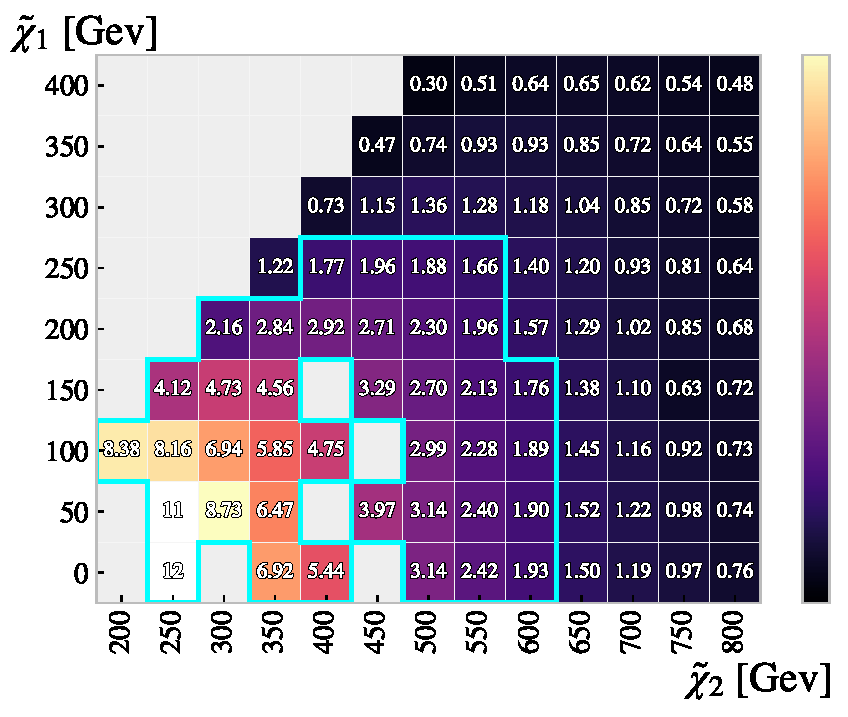
\includegraphics[width=\textwidth]{Figures/MLResults/NN/SUSY/Grid/FS/NN_FS_MLMGridSig.pdf}
    \end{subfigure}
    }
    \caption{A grid displaying the achieved significance on the full statistics signal set, using the signal region 
    created by the \ac{NN} network.}
    \label{fig:NN_FS_MLMGridSig}
\end{figure}
Figure \ref{fig:MaxOutPCA_FS_MLMGridSig} displays a grid presenting the sensitivity of the maxout model using the full statistics 
signal set. The data used to train this model, has been through a \ac{PCA}, and the architecture is the same as described in section \ref{subsec:arch}.
Similarly to the dense \ac{NN}, by including the full statistics, the maxout model improved performance on all combinations in the original set. 
Also, the maxout model upholds the sensitivity criteria ($>1.64$) for the same mass combinations. 
Contrary to the tests performed on the original signal set however, when using the full statics, the dense network 
outperforms the maxout model in most of the signals (74/89). A possible explanation to the shift in performance, could 
be that the dense \ac{NN} lacked the statistics when training with the original signal set. When the full statistics is included,
the dense \ac{NN} (which is deeper than the maxout model) is able to train much deeper, which in tern increases sensitivity. 
However, the maxout model outperforms the dense network for the low statistics combinations, again indicating the maxout layers
ability to increase long term memory.\\
\begin{figure}
    \makebox[\linewidth][c]{%
    \centering
    \begin{subfigure}{.85\textwidth}
        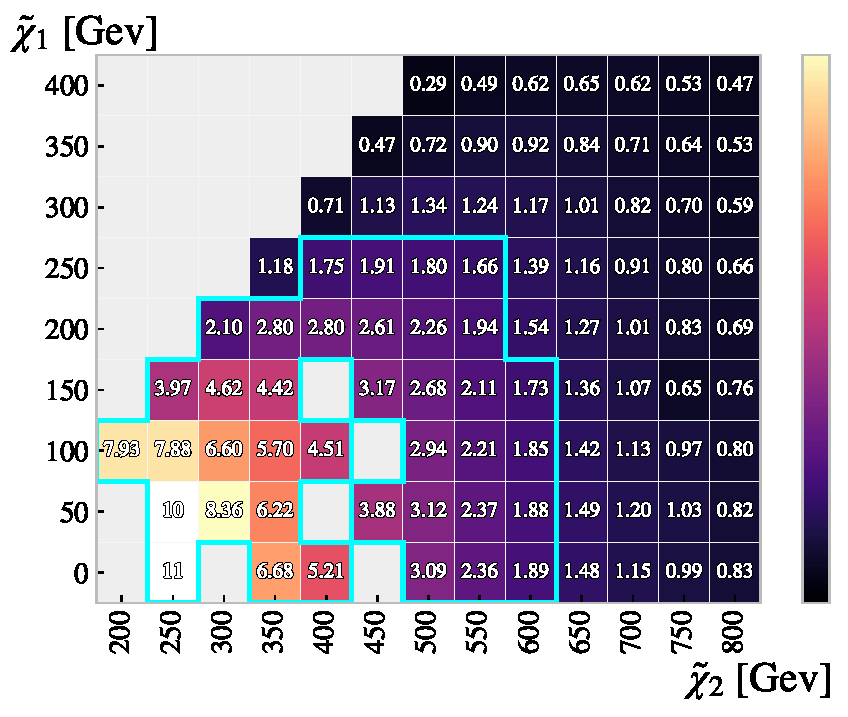
\includegraphics[width=\textwidth]{Figures/MLResults/NN/SUSY/Grid/FS/MaxOutPCA_FS_MLMGridSig.pdf}
    \end{subfigure}
    }
    \caption{A grid displaying the achieved significance on the full statistics signal set, using the signal region 
    created by the \emph{MaxOut} network.}
    \label{fig:MaxOutPCA_FS_MLMGridSig}
\end{figure}
Finally, I applied the \ac{PNN} to the full statistics signal set. The results are found in the grid presented in figure \ref{fig:PNNPCA_FS_MLMGridSig}.
Similarly to the tests performed with the original signal set, the \ac{PNN} is able to achieve an incredible sensitivity for the high statistics mass combinations
($\tilde{\chi}_2<400$). For the combinations with the highest statics ($\tilde{\chi}_2<300$), the \ac{PNN} more than doubles the achieved significance of the previous 
to methods. For the lower statistics combinations, the \ac{PNN} drops in performance. Moreover, the performance of the \ac{PNN} on the combinations with the highest 
statistics in the original signal set ([$\tilde{\chi}_1=250$, $\tilde{\chi}_2=400$GeV] and [$\tilde{\chi}_1=200$, $\tilde{\chi}_2=450$GeV]), has decreased by more than half.
This is an indication that including further trends in the data was destructive for training. In other words, although the \ac{PNN} achieves impressive sensitivity towards high 
statistics mass combinations, it suffers from the lack of long term memory which allows the maxout model to uphold performance for lower statics combinations. 
Finally, in comparison to the ordinary dense network and the maxout model who both achieved sufficient sensitivity for 38/89 combinations, the \ac{PNN} only did so for 33/89.\\
\begin{figure}
    \makebox[\linewidth][c]{%
    \centering
    \begin{subfigure}{.85\textwidth}
        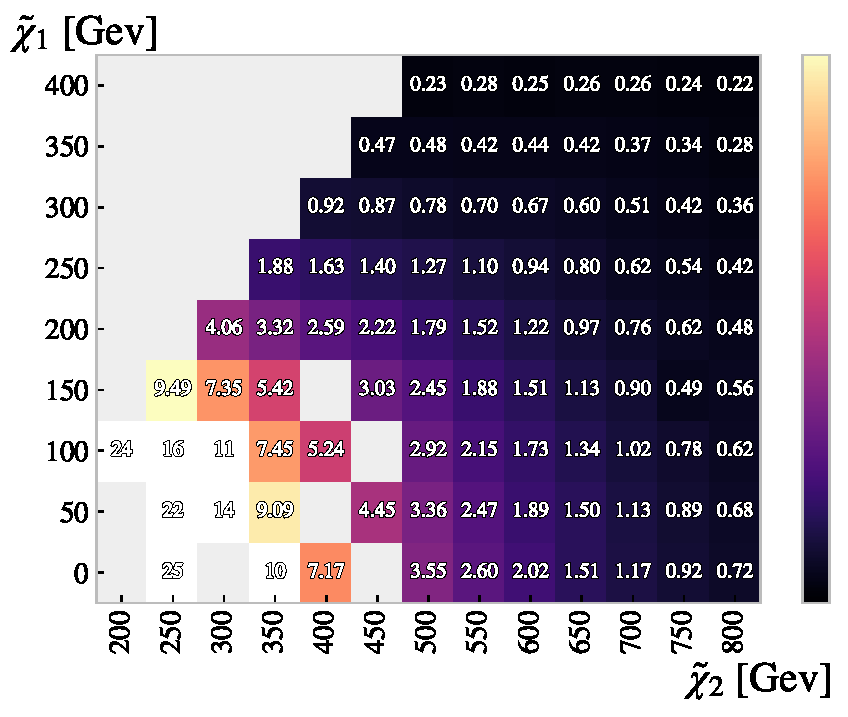
\includegraphics[width=\textwidth]{Figures/MLResults/NN/SUSY/Grid/FS/PNNPCA_FS_MLMGridSig.pdf}
    \end{subfigure}
    }
    \caption{A grid displaying the achieved significance on the full statistics signal set, using the signal region 
    created by the \emph{PNN} network.}
    \label{fig:PNNPCA_FS_MLMGridSig}
\end{figure}
To summarize the comparisons on the full statistics signal set, I created a pie-plot in figure \ref{fig:FSComp}. As shown in the figure, the ordinary dense \ac{NN}
achieved the highest sensitivity in most of the combinations (49/89), followed by the \ac{PNN} (25/89) and the maxout model (15/89). From the tests we can conclude that 
the \ac{PNN} network achieves the highest sensitivity, but struggles for unbalanced data sets. On the contrary the ordinary dense neural network performs best with larger amounts of 
training data, achieving the highest sensitivity on the most amount of combinations, but never attains the same degree of sensitivity as the \ac{PNN}. The maxout layer underperforms on 
most combinations, but exhibits impressive training memory when attaining the highest significance on the lowest statistics combinations.
\begin{figure}
    \makebox[\linewidth][c]{%
    \centering
    \begin{subfigure}{.85\textwidth}
        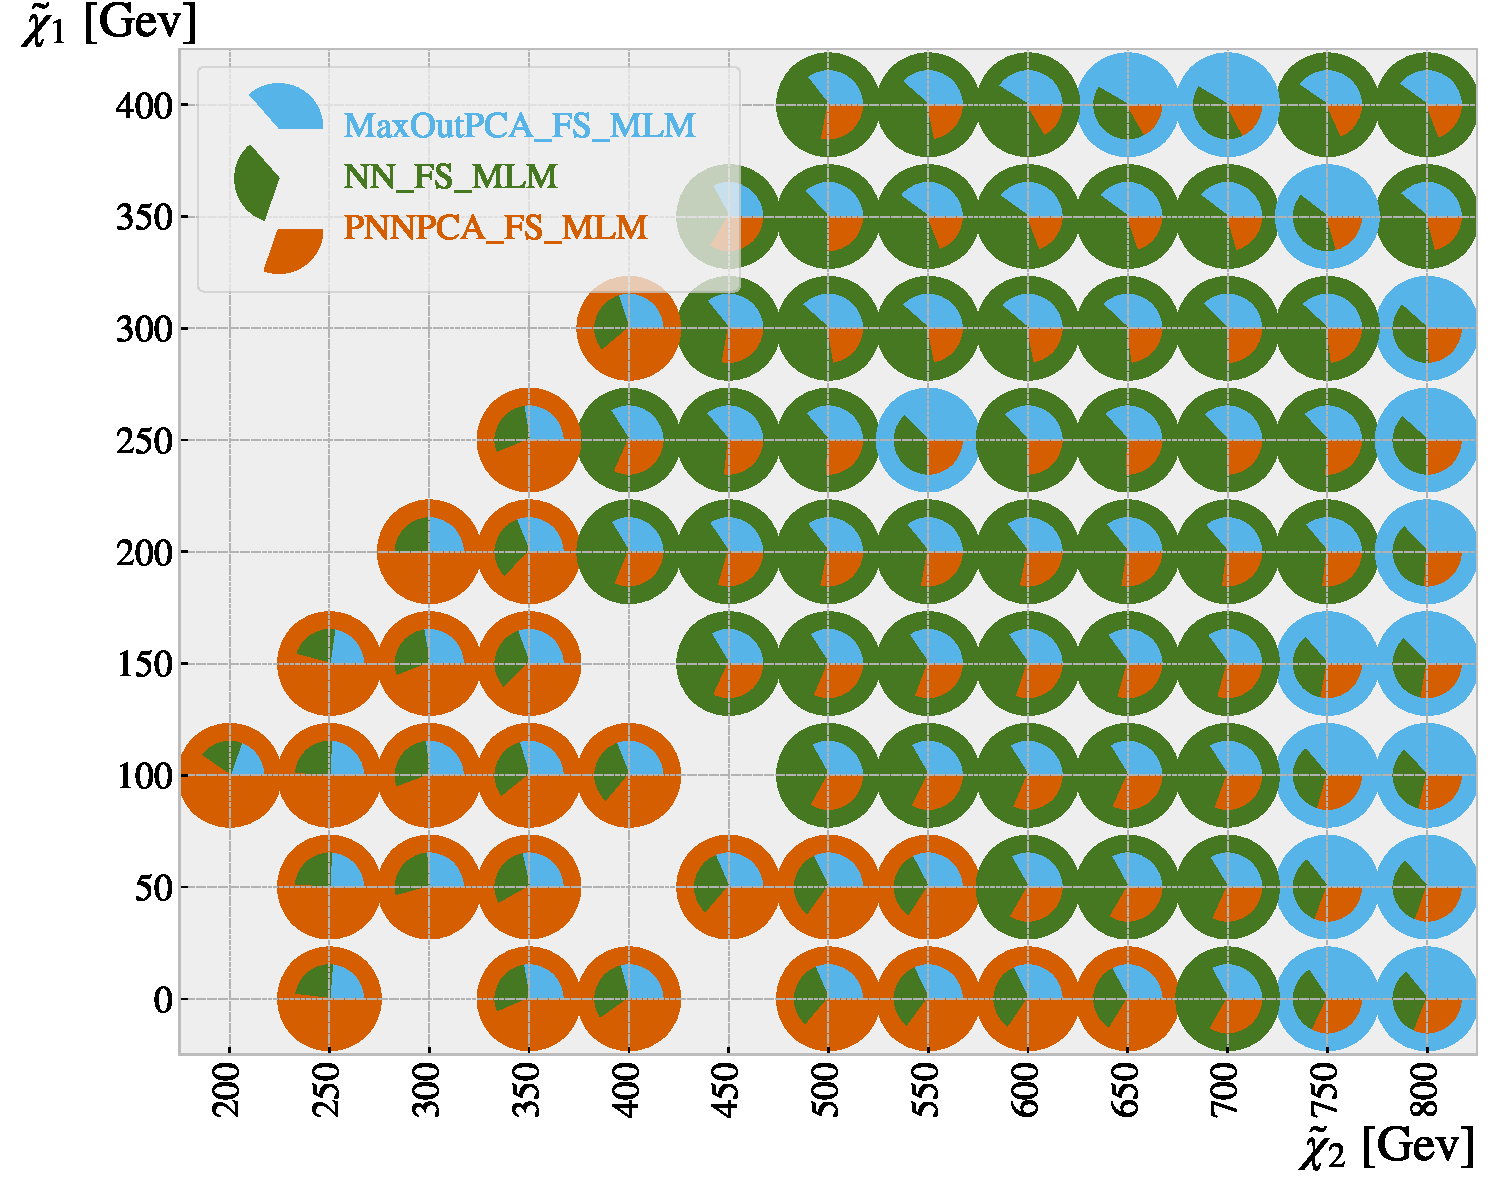
\includegraphics[width=\textwidth]{Figures/MLResults/NN/SUSY/Comparison/FS_MLMNetworkComp.pdf}
    \end{subfigure}
    }
    \caption{A grid displaying the achieved significance on the full statistics signal set, using the signal region 
    created by the \emph{PNN} network.}
    \label{fig:FSComp}
\end{figure}